\section*{Reduced Model}
\addcontentsline{toc}{section}{Reduced Model}

The initial model by Wang\cite{wang2002probabilistic} used  $N_{E} = 1600$ and $N_{I} = 400$ leaky-and-integrate spiking neurons to simulate the model. Inorder to analytically study this model, Wong et. al. \cite{wong2006recurrent} reduced it to a two variable model. Inorder to achieve this reduction, the following steps were undertaken-\\

1. The first step in this reduction is to reduce the entire population of 2000 neurons to a population consisting of 4 units namely 2 discriminatory excitatory units, 1 non selective unit and 1 inhibitory unit. Wong used mean field approach to achieve this. In order to apply the mean field approach, proper estimation of the firing activity of the population and the synaptic input currents were made. First, the driving force of the synaptic input currents has been considered to be constant (Brunel \cite{brunel2000dynamics}). Second, the contribution to the variance of the membrane potential is driven by external input to the population (the all-in-all connectivity within the neurons averages out the inter neuron contribution) as suggested by Renart et. al \cite{renart2003mean}. The $\sigma$ is fixed at constant. Finally, the firing rate was expressed by the simplified input-and-output function (Abott and Chance \cite{abbott2005drivers}):-\\

\indent $r = \phi(I_{syn}) = \frac{C_{E,I} I_{syn} - I_{E,I}}{1 - exp[g_{E,I}(c_{E,I}I_{syn} - I_{E,I})]}$\\

Here, $\phi$ is the function of the total synaptic input current $I_{syn}$ of a single cell. E,I represent either the excitatory or inhibitory neurons. $c_{E,I}$ is the gain factor and $g_{E,I}$ is the noise factor that determines the shape of the curvature of $\phi$ (which is linear threshold function for large g). This simplified model was derived from the first passage time formula of a single cell LIF model driven by a AMPA receptor mediated external gaussian noise. \\

Using this simplications and estimations, the entire neural population was able to be converted into 4 units (as mentioned initially). These units can be represented by 11 variables, mentioned below :-\\

\indent $\tau_{r} \frac{dr_{i}}{dt} = -r_{i} + \phi(I_{syn,i})$\\

\indent $\tau_{r} \frac{dr_{I}}{dt} = -r_{I} + \phi(I_{syn,I})$\\

\indent $\frac{S_{AMPA,i}}{dt} = - \frac{S_{AMPA,i}}{\tau_{AMPA}} + r_{i}$ \\

\indent $\frac{dS_{NMDA,i}}{dt} = - \frac{S_{NMDA,i}}{\tau_{NMDA}} + (1 - S_{NMDA,i})F(\psi(r_{i}))$ \\

\indent $\frac{dS_{GABA}}{dt} = - \frac{S_{GABA}}{\tau_{GABA}} + r_{I}$ \\

Here, $i = 1,2,3$ represent the 3 units namely 2 stimuli discriminatory excitatory neuron and 1 unit of non selective excitatory neuron. $I$ is the inhibitory unit. $r_{i}(t)$ and $r_{I}$ are the mean firing rate of the excitatory and inhibitory units. S is the synaptic gating variable and $\tau$ is the decay time constant. \\ 

2. Using the mean field approach, the model is represented by 11 variables. This model can be further reduced into 8 variables by observing the activity of the non selective excitatory unit. As the firing rate of the non selective unit is more or less constant, it can be replaced by a constant mean rate of 2 Hz. However, this simplification does introduce certain consequences. The first being the difference between the previous model and the current model's firing rate is about 1 Hz. The second consequence is that we would neglect the slightly increased inhibition on the selective excitatory unit by the slightly elevated activity of the non selective unit.

Additionally, the inhibitory interneurons can be linearised as the instantaneous firing rate ~8 Hz and the mean firing rate ~ 8 to 15 Hz meakes the single cell input-output relation linear which can be expressed as :-\\

\indent $\phi (I_{syn}) = \frac{1}{g_{2}}(c_{I} I_{I}) + r_{0}$ \\

The self inhibitory coupling term lowers the effective firing rate by a factor of $1 + (c_{I}/ g_{2})J_{II}$. This removes the self consistancy calculation of the inhibitory population. \\

3. The final reduction of the neural model was achieved by analysing the time membrane constant of the neurons and the gating variables. The membrane time constant of an instantenous cell can be ignored as the firing rate of a cell is instantenous [Brunel et. al. \cite{brunel2001effects} and \cite{fourcaud2002dynamics}]. Among the gating variables, $S_{NMDA}$ has the longest time decay and hence dominates the time evolution of the system. The gating NMDA variable is defined as:- \\

\indent $\frac{dS_{NMDA,i}}{dt} = - \frac{S_{NMDA,i}}{\tau_{NMDA}} (1 - S_{NMDA,i})F(\psi_{i})$\\

Where, i represents the two excitatory stimuli discriminatory units and $S_{NMDA}$ is the gating variable of NMDA receptor and $\tau_{NMDA}$ is the time membrane constant of that receptor.\\

The above estimations finally reduced the 2000 spiking neurons into a two variable model, defined as :-\\

\fbox{\begin{minipage}{20em}
\indent $ \frac{dS_{1}}{dt} = G_{1}(S_{1}, S_{2}) = - \frac{S_{1}}{\tau_{S}} + (1 - S_{1}) \gamma H(x_{1}, x_{2}) $

\indent $ \frac{dS_{2}}{dt} = G_{2}(S_{2}, S_{1}) = - \frac{S_{2}}{\tau_{S}} + (1 - S_{2}) \gamma H(x_{2}, x_{1}) $
\end{minipage}}\\

Here, $H(x_{1},x_{2})$ and $H(x_{2},x_{1})$ are the firing rate of the two units. Again, $x_{1}$ and $x_{2}$ is defined as:-\\

\indent $x_{1} = J_{N, 11} S_{1} - J_{N, 12} S_{2} + I_{0} + I_{1} + I_{noise,1}$

\indent $x_{2} = J_{N, 22} S_{2} - J_{N, 21} S_{2} + I_{0} + I_{1} + I_{noise,2}$

\begin{multicols}{2}
\begin{center}
  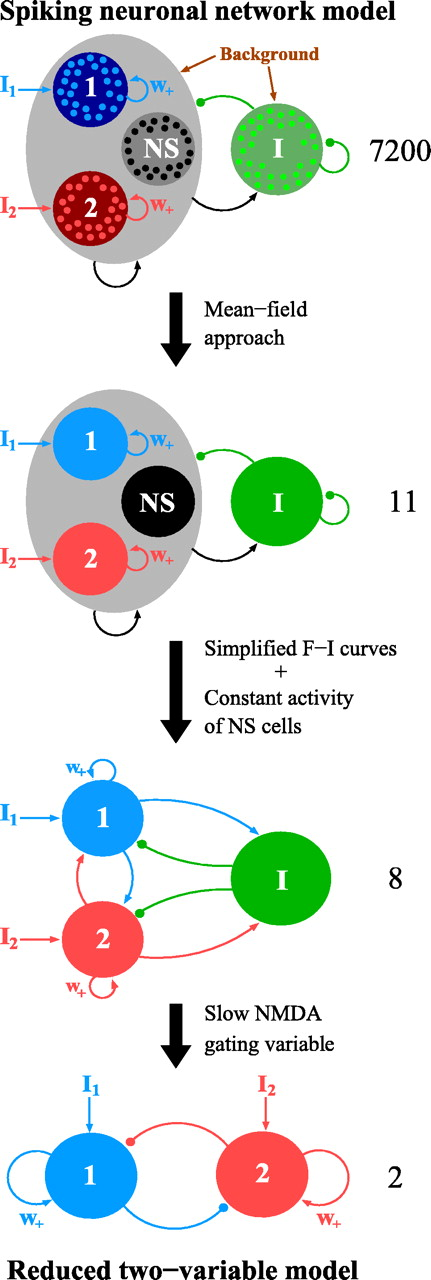
\includegraphics[width=55mm,scale=0.1]{fig/Model.jpg}
  \label{fig: Reduction model}
\end{center}

$I_{noise,i}$ is the noise term. $I_{0}$ is the common external input to both population. $S$ is the gating variable. $J_{N,ij}$ are the effective coupling constants. $Fig 2$ shows the entire reduction process.
\end{multicols}












